\chapter{Angular sensing and control characterization and performance in the radiation pressure eigenbasis} 

\label{ch:characterization}




% In this chapter I show how the angular displacements are sensed and
% why control filters implemented in the eigenbasis of radiation
% pressure torques is best. 



% \section{Sensing}
% There are five main subsets of sensor systems for the ASC:
% \begin{itemize}
% \item OSEMs
% \item optical levers (MMT3, RM, BS, ITMX, ITMY, ETMX, ETMY) \vspace{-10pt}
% \item camera image (BS)
% \item quadrant photodiodes (QPDX, QPDY) \vspace{-10pt}
% \item wavefront sensors (WFS1, WFS2, WFS3, WFS4) \vspace{-10pt}
% \end{itemize}
% Together, these sensors need to provide enough information to derive
% adequate control signals for 9 mirrors in both pitch and yaw. Both
% absolute motion (AC) and relative motion (DC) need to be
% suppressed. The OSEMs and optical levers provide local AC control to
% the mirrors. The video camera and the QPDs control the pointing of the
% input beam; the video camera works at DC and the QPDs at both DC and
% AC. The WFS provide the top level fine tuning of DC and AC control to
% the 5 main mirrors.


% \subsection{OSEMs}
% The most basic level of control is local damping of each suspended
% optic provided by the OSEMs. This is always on, even when the
% interferometer loses lock. It works by sending current through the
% OSEM coils to keep a constant amount of light on the OSEM shadow
% sensor.


% \subsection{Optical levers}
% The optical levers are local to each large optic and provide a record
% at all times of pitch and yaw pointing of each mirror with respect to
% the ground. The mirrors are velocity-damped only by the optical
% levers; they are not controlled at DC. The optical lever is a HeNe
% laser beam that reflects off of the mirror and onto a QPD. Both the
% laser and QPD are mounted on heavy piers to reduce the seismic noise
% contribution to the QPD signal. The optical lever provides a feedback
% signal to the mirror's coils to reduce the sensed motion. Each large
% optic has its own independent optical lever loop which is almost
% always on, even when the interferometer is out of lock. The optical
% lever loops provide the second level of controlled stabilization of
% the mirrors, after only the local damping.


% \subsection{Camera image}
% The most primitive sensor is that of the physical video camera.  The
% video camera monitors the location of the spot on the beam splitter,
% thus serving as a sensor of the pointing of the input beam. The image
% of the speckle of light reflected off of the beam splitter (see
% Fig. \ref{fig:BCS}) is fed into a labview program which integrates the
% intensity of the image to identify the coordinates of the center of
% the beam spot. This is compared with a hardcoded desired center
% location and a mirror upstream, MMT1 is moved to redirect the input
% beam, minimizing the difference between the desired and actual beam
% spot location on the BS.

% \begin{figure}
% \begin{centering}
% 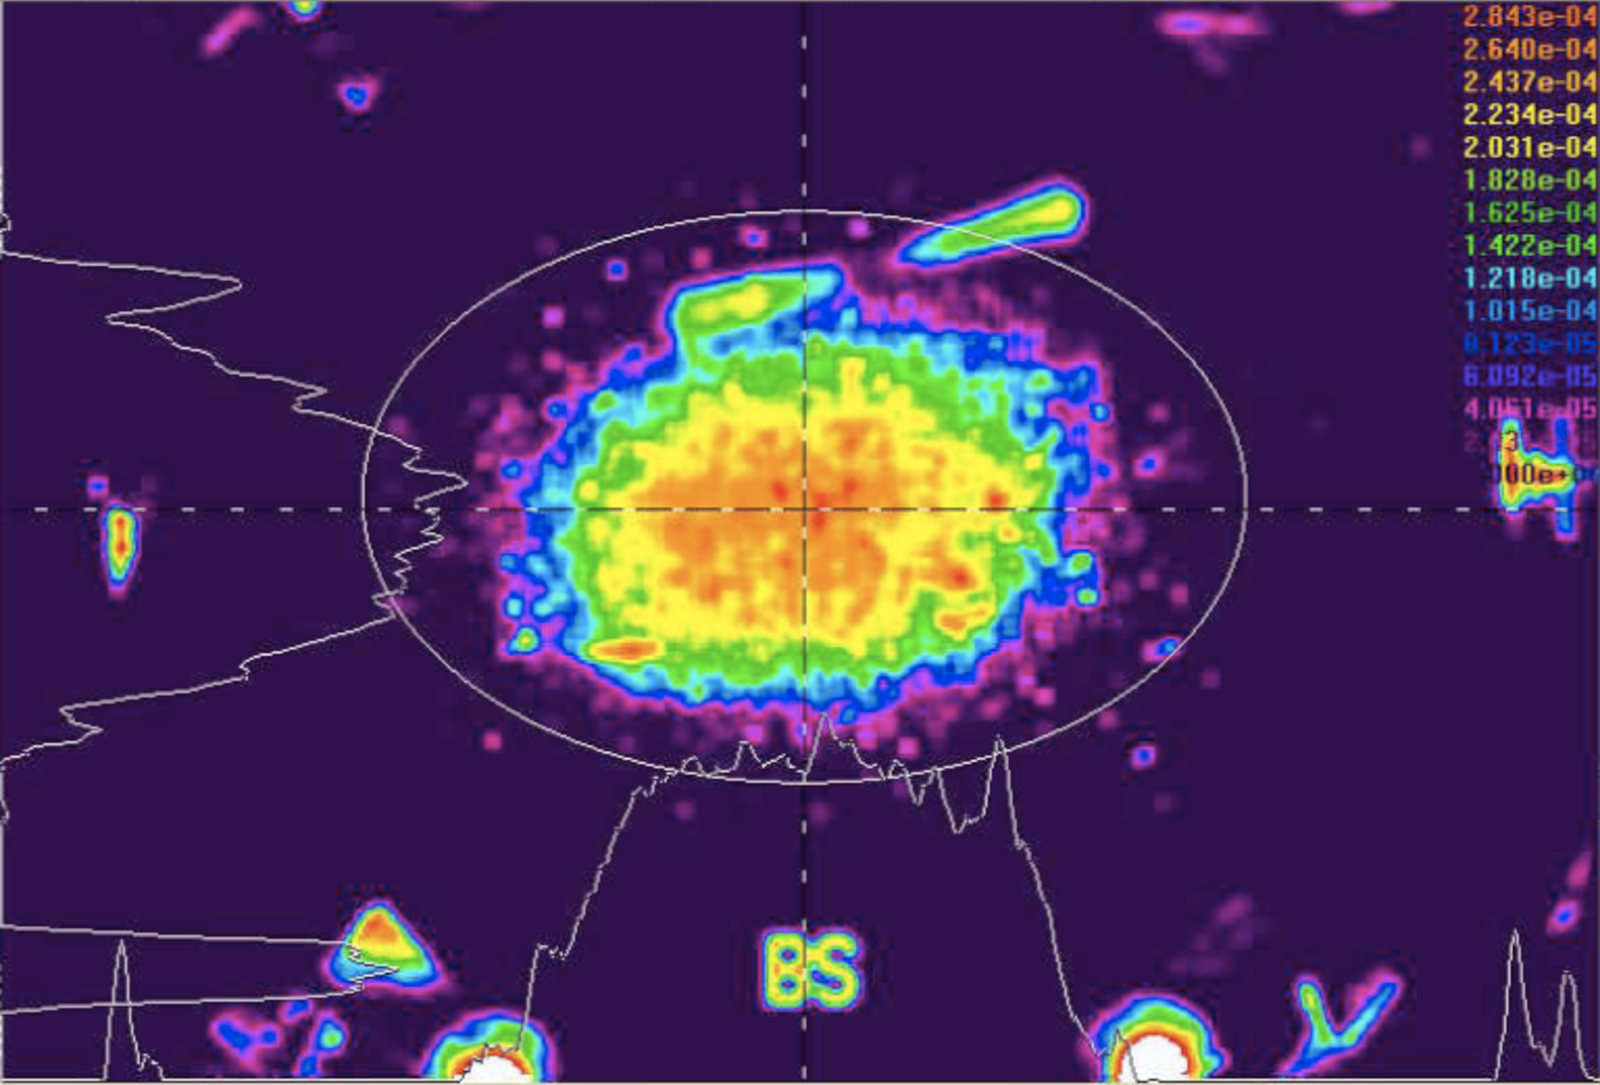
\includegraphics[width=0.8\textwidth]{figures/BCSspiricon.pdf}
% \caption{Image of beam on beam splitter as used for the beam centering servo.}
% \label{fig:BCS}
% \end{centering}
% \end{figure}


% \subsection{QPDs}  
% QPDX and QPDY see the small amount light that is transmitted through
% the ETMs, providing a monitor of the modal axes of the arm cavities. Together with the , they maintain the alignment of the input . QPDX 


% \subsection{WFSs}  
% The wavefront sensors provide the most sophisticated form of
% measuring angular motion of the mirrors. Their frame of reference is
% the fundamental Gaussian mode of the interferometer cavities (x-arm,
% y-arm, recycling cavity) as aligned to ???. All of the mirrors
% globally follow the pointing of the input beam (via the QPDs) which is
% in turn stabilized to the center of the beam splitter (via the BCS) at frequencies well
% below the pendulum resonances. The job of the wavefront sensors is to
% keep the mirrors aligned to one another up to several Hz within this
% hierarchy of alignment. The WFS provide DC and AC control to the
% mirror angles. 




% \section{Control}
% When the gain is really high, comparing the calibrated error and
% control signals shows just what the control loop is doing. The error
% is the residual and the control is what there would be without the
% loop.

% error * (1+G) is the motion without the loop, where G is the open loop gain.

% \begin{itemize} 
% \item optical lever calibration
% \item residuals, perhaps for different kinds of seismic
% \item compare to mirror motion with no ifo (demonstrate ASC suppression)
% \end{itemize}

% \textcolor{blue}{This intro is a work in progress! Set up reader to
%   hear about measurements of the Enhanced LIGO system.}
% The basis for angular control in Initial LIGO was the sensor
% basis. The wavefront sensors are located such that they sense
% common/differential ETM/ITM angular motion and the filters were
% designed to feed back to those sets of motions. This does not, however,
% lend itself to easily handling radiation pressure torque. Since the
% WFS basis is not the radiation pressure eigenbasis of Section
% \ref{sec:eigenbasis}, each control servo handled combinations of the
% soft and hard modes. Due to radiation pressure, each mirror has two
% resonances, a more complicated plant than that offered by the
% eigenbasis which has a single resonance for each mode.


The meat of the Enhanced LIGO ASC upgrade was to switch the control
servo from the sensor basis to the natural radiation pressure
eigenmode basis, and to keep the contamination to DARM at a minimum. I
present in this chapter the design of the new basis and measurements I
made to characterize it and its effect on DARM.

A critical aspect of the characterization of any system is to
calibrate the data in physical units to facilitate comparison to
models and to make meaningful statements. Since the LIGO data is
collected digitally, the units are naturally in digital counts. Part
of my work was therefore to calibrate each of the relevant ASC
channels to physical units. I include the details of the calibrations
in Appendix~\ref{ch:ASCcal}.

Also, as shown in Sec.~\ref{sec:oplevspectra} almost all of the mirror
motion is in fact due to the ground. Therefore, the measurements I
made of the ASC are very sensitive to the particular state of seismic
noise. I include in Appendix \ref{sec:groundmotion} seismic spectra
from the time of each measurement I present.




\section{The ASC Change of Basis}
The change in control basis from Initial LIGO to Enhanced LIGO was a
rather straightforward operation of changing only the ASC input matrix
and the ASC output matrix, as shown in Fig.~\ref{fig:ASCcontrolservo} and
described in the following subsections.

The convention for the naming of the WFS control signals is WFS1,
WFS2A, WFS2B, WFS3, and WFS4, as seen in the channel names. This can
be misleading because of the similarity to the sensor names (WFS1Q,
WFS2I, WFS2Q, WFS3I, and WFS4I), potentially leading one to assume a
one-to-one correspondence. For clarity in this dissertation, I refer
to the WFS control signals by the radiation pressure eigenbasis
degrees of freedom they represent: 
\begin{itemize}
\item differential soft (dSoft) \\
\item common soft (cSoft) \\
\item differential hard (dHard) \\
\item common hard (cHard) \\
\item recycling mirror (RM)
\end{itemize}
Because each mode (for both pitch and yaw) has two possible
directions, differential and common refer to the comparison of the
sign of the mode in each arm.

%\textcolor{blue}{make block figure!}



\subsection{WFS Input Matrix}
%\textcolor{blue}{(Move optical gain discussion somewhere else?)}
Optical gain is a term used in LIGO to described the amount of laser
power produced at some interferometer port for a given physical change
of some aspect of the interferometer. Ideally, photodiodes are placed
where the optical gain is high. For the case of the wavefront sensors,
one is placed at the anti-symmetric port where differential-mode
signals are transmitted, one is placed to look at a pick-off of the
beam in the recycling cavity which contains common and differential
information, and two are placed at the reflected port, where
common-mode signals end up. The precise locations are determined from
the Gouy phases of the light. Details are found in
Ref.~\cite{Barsotti2009Modeling}. 

The WFS optical gain is a measure of how much TEM01/TEM10 mode shows
up at the locations of the wavefront sensors when a mirror (or
specific combination of mirrors) moves in angle. Given the wavefront
sensor is designed to measure the amplitude of this higher order mode,
its error signal conveys the optical gain.
% include subtlety of pick-off fractions at ports?

The optical gain for each of the optics' motions is not concentrated
at any one particular port, although it can appear more strongly in
one location compared to another. In order to make use of as much of
the information as possible, we must use all sensors that witness a
particular motion. However, when there are multiple signals at a
particular place, the WFS error signals tell us the sum of all optical
gains at its location. The amount of optical gain at each detector for
each motion at one particular frequency forms the \emph{sensing
  matrix}. The inverse of the sensing matrix is known as the
\emph{input matrix}, which tells how to take the appropriate weighted
sum of signals in order to reconstruct a particular motion. The
procedure for measuring the sensing matrix is as follows:
\begin{enumerate}
\item excite one of the mirrors (or specific combination of mirrors)
  at frequency $f$ \vspace{-10pt}
\item demodulate each of the WFS signals at $f$ \vspace{-10pt}
\item normalize to the phase of the excitation readback \vspace{-10pt}
\item repeat for each mirror (or sets of mirrors)
\end{enumerate}
A key aspect of the measurement is that a notch filter at frequency
$f$ is engaged so the control servo does not suppress our excitation.

An example calibrated sensing matrix in the radiation pressure
eigenbasis as taken during a 10~W lock 
% April 14, 2010 
is shown in Table \ref{table:sensing}. Rows represent excitation and
columns are the wavefront sensors.  Before inverting to create the
input matrix, the smallest of the elements (which are more or less
equivalent to the elements for which optical gain is also expected to
be weak), are artificially set to zero. This avoids the contamination
of strong signals by those with weak signal-to-noise ratios. The
elements that remain after this process are highlighted by boxes. Note
that the sensing matrix is in fact composed of two sub-matrices: one
for the differential degrees of freedom, and one for the common
degrees of freedom. Also, WFS1Q has particularly strong signal
compared to the other wavefront sensors. We see in
Sec.~\ref{sec:WFSolgs} that this allows us to provide much more
control to the differential soft mode compared to the other modes.

\begin{table}
\centering
\caption[WFS optical gain matrix]{Optical gain at 9.7~Hz in units of
  Volts per degree of freedom microradian (pitch). Numbers in
  \textcolor{gray}{gray} are the measurement results that have
  coherences less than 0.9. Boxes highlight the elements actually used
  in the control system. All other elements are set to zero.}
\begin{tabular}{l l l l l l}
\hline
WFS1Q & WFS2Q & WFS2I & WFS3I & WFS4I &  \\
\hline
\fbox{2.0}   & \textcolor{gray}{0.03} &\textcolor{gray}{0.06} & \textcolor{gray}{-0.008}  &  \textcolor{gray}{0.01} & dSoft \\
\fbox{0.31}  & \fbox{-0.03} &\textcolor{gray}{-0.04} &  \textcolor{gray}{0.002} & \textcolor{gray}{-0.01} & dHard \\
   \textcolor{gray}{0.02} & \textcolor{gray}{-0.01} &  \fbox{0.18} & \fbox{\textcolor{gray}{-0.02}} &  \fbox{\textcolor{gray}{-0.10}} & cSoft \\
   \textcolor{gray}{0.17} & \textcolor{gray}{-0.01} & \fbox{-0.21} &  \fbox{\textcolor{gray}{0.007}} & \fbox{-0.12} & cHard \\
   \textcolor{gray}{0.09} & \textcolor{gray}{-0.01} & \fbox{-0.21}  &  \fbox{0.04} & \fbox{-0.21} & RM \\
\hline
\end{tabular}
\label{table:sensing}
\end{table}

% \begin{table}
% \centering
% \caption[WFS optical gain matrix]{Optical gain at 9.7~Hz in units of WFS counts / dof radian
%   (pitch). Numbers in \textcolor{gray}{gray} are the measurement
%   results that have coherences less than 0.9. Boxes highlight the
%   elements actually used in the control system. All other elements are
%   set to zero. \textcolor{blue}{change to Volts!}} 
% \begin{tabular}{l l l l l l}
% \hline
% WFS1Q & WFS2I & WFS2Q & WFS3I & WFS4I &  \\
% \hline
% \fbox{5.8e+12}   & \textcolor{gray}{3.3e+09} &\textcolor{gray}{6.7e+09} & \textcolor{gray}{-1.3e+09}  &  \textcolor{gray}{2.2e+09} & dSoft \\
% \fbox{9.2e+11}  & \fbox{-3.7e+09} &\textcolor{gray}{-4.0e+09} &  \textcolor{gray}{3.4e+08} & \textcolor{gray}{-1.7e+09} & dHard \\
%    \textcolor{gray}{5.4+10} & \textcolor{gray}{-1.3e+09} &  \fbox{2.1e+10} & \fbox{\textcolor{gray}{-3.9e+09}} &  \fbox{\textcolor{gray}{-1.7e+10}} & cSoft \\
%    \textcolor{gray}{4.9e+11} & \textcolor{gray}{-1.6e+09} & \fbox{-2.4e+10} &  \fbox{\textcolor{gray}{1.2e+09}} & \fbox{-1.9e+10} & cHard \\
%    \textcolor{gray}{2.6e+11} & \textcolor{gray}{-1.1e+09} & \fbox{-2.4e+10}  &  \fbox{7.0e+09} & \fbox{-3.5e+10} & RM \\
% \hline
% \end{tabular}
% \label{table:sensing}
% \end{table}

%\textcolor{blue}{Paragraph discussing sensing matrix numbers.}



\subsection{WFS Output Matrix}
The WFS output matrix determines how to convert the radiation pressure
eigenbasis control signals into individual mirror control signals. It
is the basis transformation matrix, $S$, as defined in
Eq. \ref{eq:S}. The matrix is arbitrarily normalized so the largest
element is $1$, and it is repeated with appropriate sign changes to
form differential and common soft and hard modes of the two arms. The
output matrix is shown in Table \ref{table:output}, where the $r$ is
0.91 for Livingston and 0.87 for Hanford. 

\begin{table}
\centering
\caption[WFS output matrix]{WFS output matrix (pitch). For the Livingston cavity geometry
  $r=0.91$ and for Hanford $r=0.87$.}
\begin{tabular}{l l l l l l}
\hline 
dSoft & dHard & cSoft & cHard & RM & \\
\hline 
1 & r & 1 & r & 0 & ETMX\\
-1 & -r & 1 & r & 0 & ETMY \\
r & -1 & r & -1 & 0 & ITMX\\
-r & 1 & r & -1 & 0 & ITMY\\
 0 & 0 & 0 & 0 & 1 & RM\\
\hline
\end{tabular}
\label{table:output}
\end{table}


\subsection{Diagonalizing the WFS Drive Matrix}

%\textcolor{blue}{fix this} 
During the sensing matrix measurement, the optical levers provide a
record of the motion of the test masses. I combined the
optical lever responses (via the output matrix, Table~\ref{table:output})
to determine the amplitude of each radiation pressure degree of freedom's
movement. The actual numbers for the measurement data presented in
Table~\ref{table:sensing} are found in Table~\ref{table:excitations_calibrated}.

This matrix tells the extent to which the ASC control matrix excites
the degree of freedom it is designed to excite. Columns are
excitations and rows are the pitch motions at 9.7~Hz in units of
\microrad. Ideally, this would be a diagonal matrix and it is up to at
most a factor of two. I had to calculate modifications to the output
matrix in order to achieve the eigenbasis motion matrix as diagonal as
this one. The modifications take the form of gains to the mirror
drives and are shown in Table~\ref{table:mirrorgains}. The 30\%
difference with the model is a result of uncertainty in the cavity
$g$-factors.


% This now allows us to complete the
% first part of obtaining an optical gain matrix. Each row of the
% sensing matrix should be divided by the amplitude of that dof's
% excitation, the diagonal elements of Table
% \ref{table:excitations_calibrated}. The result of doing so gives the
% angular optical gain of the interferometer in terms of WFS digital
% counts per radian.


%\textcolor{blue}{write out the rest of this section}
% D = 'drive' = DOF excitation to DOF excited matrix (theta\_dof)
% U = 'unknown' = hardware mostly; coils, etc.
% M = 'mirror' = mirror gains; a diagonal matrix
% C = 'control' = ASC output matrix

% We have D = U*M*C. A drive is multiplied first by the output matrix (C),
% then by the mirror gains (M), then put into hardware (U) to create what's
% actually exicted.

% To make D diagonal, we want to find a new M, M\_new, which must have the
% property M\_new = inv(U)*inv(C) = M*C*inv(D)*inv(C)


\begin{table}
\centering
\caption[Actual eigenbasis motion during sensing matrix excitations]{Actual eigenbasis motion during sensing matrix excitations as
  witnessed by the optical levers. Columns are excitations and rows are
  the pitch motions at 9.7~Hz in units of \microrad. Ideally, this
  would be a diagonal matrix. It mostly is.}
\begin{tabular}{l l l l l l}
\hline
dSoft & dHard  & cSoft & cHard & RM & \\
\hline
   \textbf{5.1e-06} & -5.2e-08  & 6.1e-07 & -3.8e-08 &  -1.8e-07 & dSoft\\
  -3.4e-07 &  \textbf{5.0e-06}  &  7.3e-07 & -1.0e-06 &  2.4e-07 & dHard\\
  -4.1e-07 & -3.3e-08 &  \textbf{5.9e-06} &  6.8e-07 &  2.5e-07 & cSoft\\
  -6.4e-07 & -5.9e-07 &  1.1e-06 &  \textbf{5.7e-06} &  4.7e-07 & cHard\\
  -1.6e-07 & -1.8e-06 & -5.5e-07 &   2.6e-06 &  \textbf{5.6e-06} & RM\\
\hline
\end{tabular}
\label{table:excitations_calibrated}
\end{table}



\begin{table}
\centering
\caption[Mirror gains for diagonalization of drive matrix]{Mirror
  gains for diagonalization of drive matrix.} 
\begin{tabular}{l l l l l l}
\hline
ETMX & ETMY & ITMX & ITMY & RM & \\
\hline
1.33 & 1.38 & 0.96 & 0.87 & 1.0 \\
% 1.33 & 0 & 0 & 0 & 0 & ETMX\\
% 0 & 1.38 & 0 & 0 & 0 & ETMY \\
% 0 & 0 & 0.96 & 0 & 0 & ITMX\\
% 0 & 0 & 0 & 0.87 & 0 & ITMY\\
%  0 & 0 & 0 & 0 & 1 & RM\\
\hline
\end{tabular}
\label{table:mirrorgains}
\end{table}




\section{Sensing Matrix Stability}
%\textcolor{blue}{Show how the sensing matrix changes in time (APS presentation).}
%sensing matrix stability over time, with power;
%just how diagonal is the system?

As the interferometer conditions change, so does the sensing
matrix. The inverse of the sensing matrix, the input matrix, is
hardcoded in the digital control servo and not actively
updated. Therefore, it can be expected that the ASC performance may
not be stable. 

By design, the input matrix is not exactly the inverse of the sensing
matrix, meaning the system is not completely diagonal. For example,
the input matrix times the sensing matrix is, by design:
 \[ \left\llbracket \begin{array}{ccccc}
0.79 & 0 & 0.30 & 0 & 0 \\
0 & 1.0 & 0 & 0 & 0 \\
0 & 0 & 1.0 & 0 & 0 \\
0 & 0 & 0 & 1.0 & 0 \\
0 & 0 & 0 & 0 & 1.0 
\end{array} \right\rrbracket\] 

Over time, the sensing matrix changes enough that the system is even less 
diagonal. Only 10 minutes after having measured and created the input
matrix, the product of the input matrix with a newly measured new
sensing matrix is: 
\[ \left\llbracket \begin{array}{ccccc}
0.79 & 0 & 0.32 & 0 & 0 \\
0 & 1.0 & 0 & 0 & 0 \\
-0.02 & 0 & 1.0 & 0 & 0 \\
0 & -0.02 & 0 & 1.0 & 0.02 \\
0 & 0.02 & 0 & 0.05 & 1.03 
\end{array} \right\rrbracket\] 

After one week, it is:
 \[ \left\llbracket \begin{array}{ccccc}
0.67 & 0 & 0.27 & 0 & 0 \\
0 & 0.91 & 0 & 0.03 & -0.03 \\
0.09 & 0 & 0.84 & 0 & 0 \\
0 & 0.15 & 0 & 0.83 & 0.27 \\
0 & 0.06 & 0 & 0.07 & 1.04 
\end{array} \right\rrbracket\] 

And after three weeks, it is:
 \[ \left\llbracket \begin{array}{ccccc}
1.4 & 0 & 0.55 & 0 & 0 \\
0 & 1.8 & 0 & -0.09 & 0.15 \\
-0.08 & 0 & 2.0 & 0 & 0 \\
0 & -0.22 & 0 & 1.4 & 0.64 \\
0 & 0.30 & 0 & -0.72 & 2.9 
\end{array} \right\rrbracket\] 

Despite these significant changes, the interferometer remained stable
and the sensitivity remained constant. This shows that the ASC is a
very robust sensing and control system.


\section{Input Beam Motion}
The beam centering and QPD servos operate up to only about 50~mHz,
meaning the beam-centering degree of freedom is uncontrolled at higher
frequencies. Since beam spot motion on the test masses couples to
DARM, anything that causes the beam's position on the test mass to
change on time scales faster than half a minute becomes itself a
direct noise source for DARM. The HAM seismic isolation tables from
which the input optics are suspended have resonant ``stack'' modes
from about 0.8~Hz to 3~Hz. The excess table motion at these
frequencies is transmitted to the MMTs. Jitter on the pointing of the
input beam is thus a primary contender for beam spot motion on the
test masses.

% can't move the input beam faster than the interferometer can follow it!

The wavefront servos are the mechanism by which input beam motion is
impressed on the test masses; they are responsible, among other
things, for making the interferometer follow the input beam up to
several Hz. The WFS detect differences between the angle of the cavity
(as determined by the angles of the mirrors) and the angle of the beam
impinging the cavity. If either the input beam or the cavity angle
changes, the WFS will move the mirrors to correct for the angle
mismatch. Thus, even if the mirrors are perfectly quiet, a
non-stationary input beam will result in mirror motion and mirror
motion in turn creates beam spot motion (see Eq. \ref{eq:x}).

I measured the impression of the input beam motion on the mirrors by
increasing the gain of the common-degree-of-freedom WFS servos (cHard,
cSoft, RM) for about 10~minutes. Comparing the amount of angular motion
of the mirrors as witnessed by the optical levers from this time of
high common WFS gain to a time with nominal WFS gain and similar
seismic motion, we can see the effect
directly. Fig. \ref{fig:inputbeam_impression} shows comparison
spectra, demonstrating how there is higher test mass motion around
1~Hz when the common WFS gains are higher. The rms mirror motion also
increases by about 20\%.

\begin{figure}
\begin{centering}
\subfigure{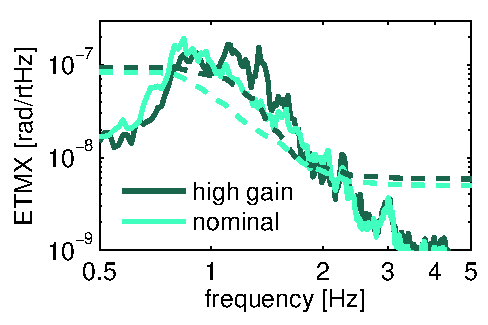
\includegraphics[width=0.5\textwidth]{figures/ETMXrms_highnom.pdf}}\subfigure{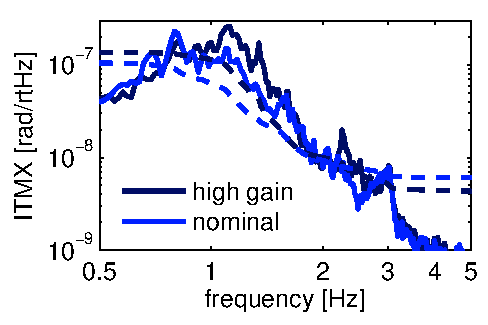
\includegraphics[width=0.5\textwidth]{figures/ITMXrms_highnom.pdf}}
\subfigure{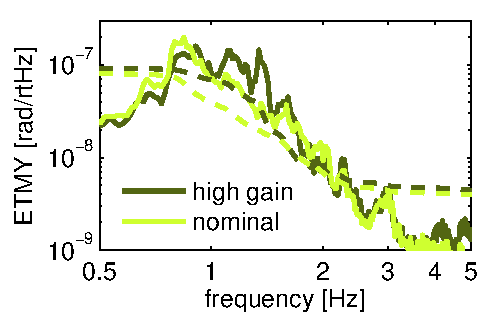
\includegraphics[width=0.5\textwidth]{figures/ETMYrms_highnom.pdf}}\subfigure{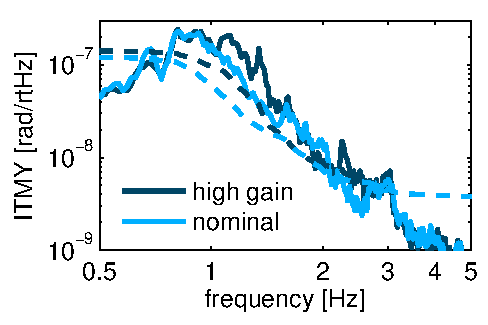
\includegraphics[width=0.5\textwidth]{figures/ITMYrms_highnom.pdf}}
\subfigure{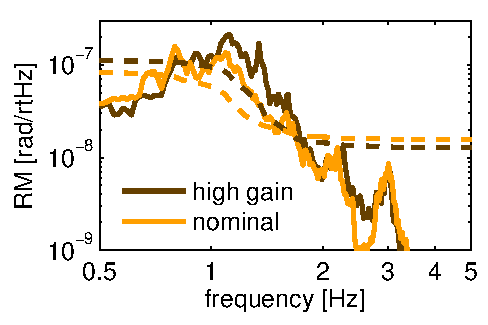
\includegraphics[width=0.5\textwidth]{figures/RMrms_highnom.pdf}}
\caption[Impression of input beam motion on the core mirrors]{Input
  beam motion impression on the core mirrors (pitch). Residual mirror
  motion as witnessed by the optical levers when the common WFS gains
  (cSoft, cHard, RM) are increased to $2.5\times$ nominal is compared
  to residual mirror motion when the WFS gains are nominal. Dased
  lines are the root-mean-square of the amplitude spectral density
  integrated from the right. Both spectra come from a time of similar
  seismic activity (typical weekday afternoon noise), shown in
  Fig. \ref{fig:seismic_highgain}.}
\label{fig:inputbeam_impression}
\end{centering}
\end{figure}

It is possible for the extra mirror motion to result from gain peaking
of the WFS servos. However, a plot of the WFS error signals during the
time of nominal gain and high gain shows that there is not, in fact,
any evidence of gain peaking. The common WFS spectra in
Fig. \ref{fig:WFS_inputbeam} do not show any extra noise when their
gains are higher. It is worth noting that the higher gain is evident
in the common WFS spectra by the extra suppression seen below
1~Hz. Also, the differential WFS spectra are unchanged, as
expected. It can therefore be concluded with reasonable certainty that
the increase in test mass motion between 1 and 2~Hz during this test
is indeed due to the WFS impressing input beam motion on the mirrors.

\begin{figure}
\begin{centering}
\subfigure{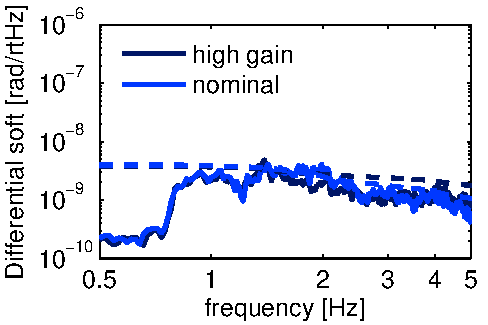
\includegraphics[width=0.5\textwidth]{figures/testWFS1_highnom.pdf}}\subfigure{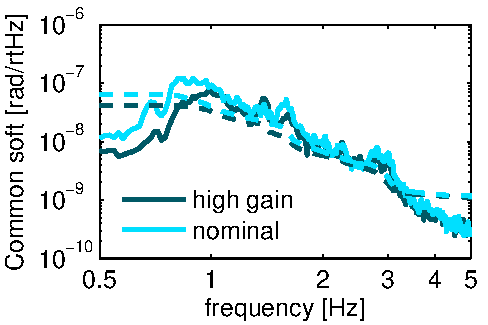
\includegraphics[width=0.5\textwidth]{figures/WFS2A_highnom.pdf}}
\subfigure{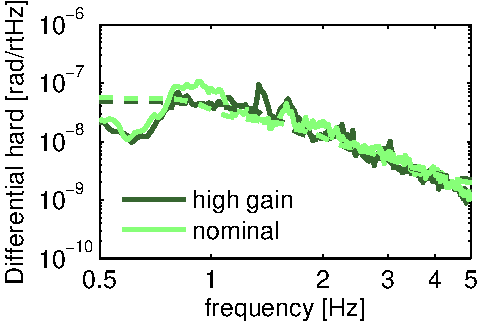
\includegraphics[width=0.5\textwidth]{figures/WFS2B_highnom.pdf}}\subfigure{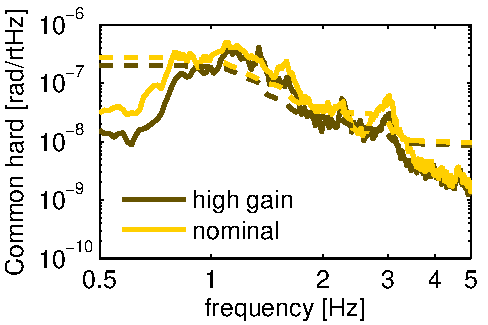
\includegraphics[width=0.5\textwidth]{figures/WFS3_highnom.pdf}}
\subfigure{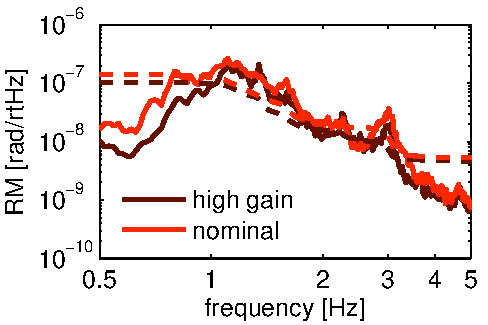
\includegraphics[width=0.5\textwidth]{figures/WFS4_highnom.pdf}}
\caption[Comparison of WFS error signals (the residual motion) during
a time of normal operation and a time when the common WFS gains were
$2.5\times$ higher than nominal]{Comparison of WFS error signals (the
  residual motion) during a time of normal operation and a time when
  the common WFS gains were $2.5\times$ higher than nominal. This
  excludes gain peaking as a cause of the extra mirror motion
  witnessed during the time of high gain. Dased lines are the
  root-mean-square of the amplitude spectral density integrated from
  the right. Fig.~\ref{fig:seismic_highgain} shows the ground motion
  spectra at the time of this measurement.}
\label{fig:WFS_inputbeam}
\end{centering}
\end{figure}


% A more quantitative study of the effects of input beam motion is to
% measure transfer coefficients between the input beam motion and the
% mirror angular (or beam spot) motion. During a full interferometer
% lock I put lines in MMT1, MMT2, and MMT3 at 1.05~Hz, 1.25~Hz, and
% 0.85~Hz, respectively, selecting excitation amplitudes large enough to
% appear in the common WFS spectra. I compared the amplitudes of the
% lines in the MMT spectra with those in the WFS spectra. The counts to
% counts transfer coefficients are shown in Table
% \ref{table:inputbeam_TFcoeffs}. Since sensing is flat, I use the shape
% of the WFS loop to extrapolate this transfer coefficient at one
% frequency to other frequencies. The result is a transfer function
% useful for making a noisebudget of input beam motion to test mass
% motion. Selecting a science mode time of typical day-time seismic
% noise, I made a noisebudget as found in Fig. \ref{fig:inputbeam_NB}.


% \begin{table}
% \centering
% \caption[MMT to WFS transfer coefficients]{MMT to WFS transfer
%   coefficients. \textcolor{blue}{Make this!!!}}
% \begin{tabular}{l l l l l l}
% \hline
%           & WFS1Q & WFS2I & WFS2Q & WFS3I & WFS4I \\
% \hline
% MMT1 & \\
% MMT2 & \\
% MMT3 & \\
% \hline
% \end{tabular}
% \label{table:inputbeam_TFcoeffs}
% \end{table}



% \begin{figure}
% \begin{centering}
% %\includegraphics[width=1.0\columnwidth]{figures/}
%   \caption[Mirror motion due to input beam impression]{Noise budget of
%     mirror motion due to input beam impression. \textcolor{blue}{Make
%       this!!}}
% \label{fig:inputbeam_NB}
% \end{centering}
% \end{figure}



\section{The Marginally-stable Power Recycling Cavity}
The power recycling cavity (PRC) is the linear cavity formed by the RM
and ITMs. Since the radius of curvature of both the RM and the ITMs
points in the same direction and the waist is well outside the
Rayleigh range of the mirrors, the cavity is geometrically
unstable. For example, in its cold state at LLO the $g$-factor of the
cavity is 1.00005 and at LHO it's 1.00003. The beam in the PRC is not
spatially contained and the cavity is degenerate with respect to
higher order modes. The heating of the ITMs from the kilowatts of
power in the arm cavities together with the ITM thermal compensation
system (TCS) serve the role of making the PRC geometrically stable for
interferometer operation. The heating and cooling of the ITMs is a
very complicated process and therefore not very precise, so the value
of the hot PRC's $g$-factor is usually not constant.

%\textcolor{blue}{differentiate magnitude of SPOB vs fluctuations in
%SPOB.} 
The changing $g$-factor has potentially severe consequences
for the ASC. Because of its geometry, the power build-up in the PRC is
very sensitve to both the mirror angles and the $g$-factor. Power
fluctuation is detrimental because the signal to noise ratios of the
sensors that probe the PRC light degrade due to the presence of
increased junk light that contributes shot noise but not
signal. WFS1Q, WFS2I, and WFS2Q are the most sensitive to the PRC
because their signals are derived from the 25~MHz sidebands. Their
sensitivity to mirror motion is therefore subject to change. Since
achieving a flat power build-up in the PRC is a difficult task (too
much motion in the PRC is quite often a cause of lock loss when making
measurements), we must update the real-time control system to reflect
their changing sensitivites. Otherwise, the mirror angles will not be
accurately controlled.

An estimate of the expected power fluctuations based on the $g$-factor
and RM motion is a straightforward excercise when using
Eq. \ref{eq:cavitydisptilt_mirrorangle} and Eq. \ref{eq:pwr_disptilt}
as derived in the Appendix. If we estimate the $g$-factors of the RM
and ITM as $g_{RM} = 1+\delta$ and $g_{ITM} = 1 - \delta$ (where
$\delta =6 \times 10^{-4}$ for LLO the cold state) and approximate the
distance of each mirror to the cavity waist as $z$ since the two
mirrors are very close to each other compared to the waist location,
then Eq. \ref{eq:cavitydisptilt_mirrorangle} reduces to:
\begin{equation}
\left\llbracket \begin{array}{c}
a_{PRC} \\
\alpha_{PRC} \end{array} \right\rrbracket = 
\left\llbracket \begin{array}{cc}
z(2+\delta)/\delta & z(2-\delta)/\delta \\
-1/\delta & -1/\delta \end{array} \right\rrbracket
\left\llbracket \begin{array}{c}
\theta_{RM}\\
\theta_{ITM} \end{array} \right\rrbracket.
\end{equation}

Fig. \ref{fig:prc_power} plots the power in the PRC as a function of
$\theta_{RM}$ for several values of $\delta$, demonstrating
the sensitivity of the PRC to the ITM heating.  For example, the
typcial RM angular displacement of $10^{-7}$ rad results in a 66\%
power loss when the PRC $g$-factor is very near instability with a
value of $1-0.0001$. Only as the $g$-factor moves further from $1$
does the angular motion of the RM have less and less of an effect on
the power build-up.

\begin{figure}
\begin{centering}
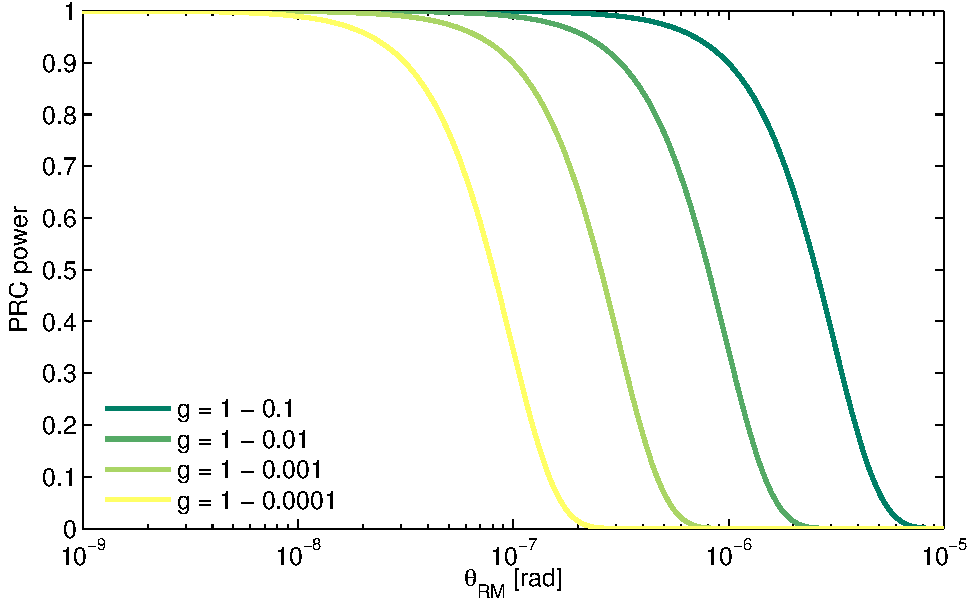
\includegraphics[width=1.0\columnwidth]{figures/prc_power.pdf}
\caption[Theoretical dependence of power recycling cavity power on
$g$-factor and mirror angle]{Dependence of power build-up in the power
  recycling cavity on the PRC's $g$-factor and the RM tilt. TCS is
  necessary for stabilizing the PRC's geometry and therefore its
  sensitivity to mirror motion. For simplicity, the ITM is assumed
  stationary in these plots.}
\label{fig:prc_power}
\end{centering}
\end{figure}


\subsection{Power Scaling}
The signal at the wavefront sensors is proportional to the amplitude
of the sidebands, or the square root of the sideband power. Thus, as
the PRC $g$-factor and therefore the power in the recycling cavity
changes, so do the WFS1 and WFS2 optical gains. In order to
compensate for this $g$-factor dependence, we multiply the WFS\{1Q,
2I, 2Q\} error signals in real-time by
\begin{equation}
\frac{1}{P_{in}} \left[\frac{\mathrm{NSPOB}}{350}\right]^{-1/2}
\end{equation}
and WFS3I and WFS4I by $1/P_{in}$. NSPOB is the normalized sideband
power in the PRC as measured by the $2f$-demodulated POB signal, and
the 350 is the reference NSPOB, treated as nominal. Thus, during
interferometer operation, all WFS signals are normalized to input
power and are not dependent on the PRC power. This correction to the
WFS signals is called power scaling.

To verify that the WFS optical gains do indeed scale with the sideband
power as expected, I tracked the WFS optical gain as $g$ changes. I
excited three of the test masses (ETMX, ITMX, RM) at three different
frequencies (9.7~Hz, 10.7~Hz, and 11.7~Hz, respectively) during a full
interferometer lock and changed the TCS settings so that over the
course of 15 minutes the $g$-factor steadily changed. Demodulating
each of the WFS signals at each of the three excitation frequencies as
a function of time shows how the strength of the signal at the WFS due
to the motion of these three mirrors changes. To compensate for the
difference in pendulum responses to the excitations, I multiplied the
demodulated signals for a particular excitation $f$ by $(f/9.7)^2$. I
also normalized the response by the phase of the mirror's motion as
witnessed by the optical levers.

The results are shown in Fig. \ref{fig:WFStrack}, and include a plot
of how NSPOB changed over time. As expected, WFS1Q, WFS2I, and WFS2Q
show dependence on the PRC power, and therefore the $g$-factor. The
WFS3 and WFS4 sensing elements are flat. Fitting lines to each of the
tracked elements, we find a good fit with the expected power of $1/2$
dependence. 

\begin{figure}
\begin{centering}
\subfigure{\includegraphics{figures/trackSPOB.pdf}}\subfigure{\includegraphics{figures/trackWFS1Q.pdf}}
\subfigure{\includegraphics{figures/trackWFS2I.pdf}}\subfigure{\includegraphics{figures/trackWFS2Q.pdf}}
\subfigure{\includegraphics{figures/trackWFS3I.pdf}}\subfigure{\includegraphics{figures/trackWFS4I.pdf}}
% \subfigure{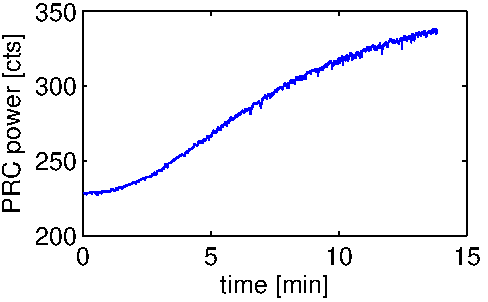
\includegraphics[width=0.5\textwidth]{figures/spob_gaintracking.pdf}}\subfigure{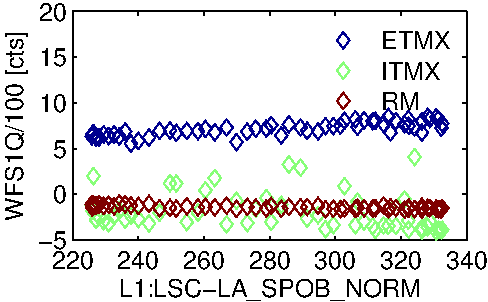
\includegraphics[width=0.5\textwidth]{figures/WFS1Q_track.pdf}}
% \subfigure{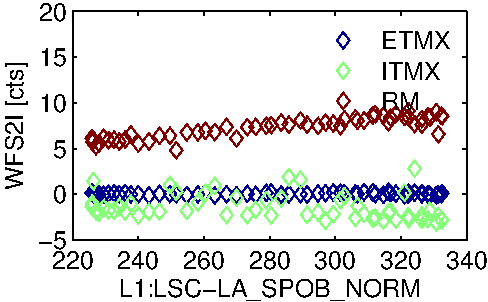
\includegraphics[width=0.5\textwidth]{figures/WFS2I_track.pdf}}\subfigure{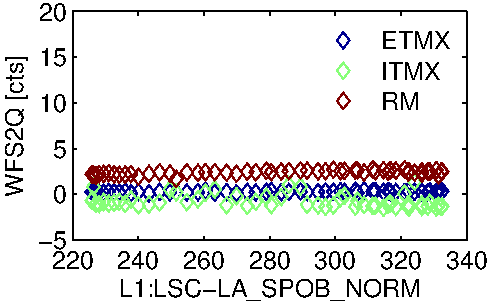
\includegraphics[width=0.5\textwidth]{figures/WFS2Q_track.pdf}}
% \subfigure{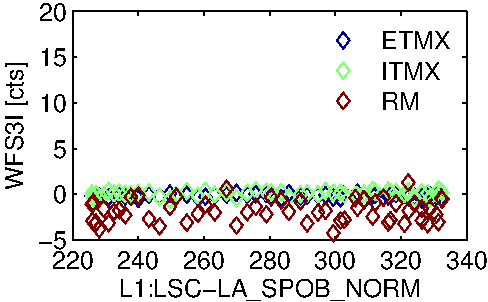
\includegraphics[width=0.5\textwidth]{figures/WFS3I_track.pdf}}\subfigure{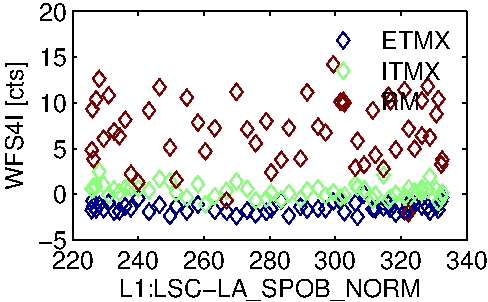
\includegraphics[width=0.5\textwidth]{figures/WFS4I_track.pdf}}
\caption[Measured dependence of the WFS error signals on the power
recycling cavity geometry]{WFS optical response to test mass motion as
  a function of power recycling cavity geometry. WFS1Q, WFS2I, WFS2Q
  are more sensitive to test mass motion as the power in the recycling
  cavity increases. Therefore, to achieve a dependable feedback
  system, we scale the error signals in real-time, forcing their
  responses to be flat with power. This range of PRC power is low for
  normal operations.}
%\textcolor{blue}{plot as ratio of first value and include fitted lines for satisfaction.}}
\label{fig:WFStrack}
\end{centering}
\end{figure}


% \subsection{Sideband imbalance}
% Another important effect of the PRC on the ASC signals is the
% balancing of the upper and lower 24.4~MHz sideband amplitudes. If
% they're not the same, then SPOB does not accurately represent the
% power in the cavity, and the WFS signals are not
% corrupted. \textcolor{blue}{(Expand.)}

% We set up a temporary optical spectrum analyzer at a pickoff of the
% anti-symmetric port beam in order to measure them. Without any TCS, we
% saw that with less than 6~W input power, the lower sideband is smaller
% than the upper sideband, at 6~W the amplitudes are equal, and above
% 6~W, the upper sideband is smaller than the lower. Thus, if TCS is not
% tuned perfectly at all times, we can expect unequal sidebands.
% \textcolor{blue}{April 1, 2009 notebook. I don't have OSA data, only
%   sketches in notebook. Worth saying anything?}



% \section{DC readout related measurements}
% \begin{itemize}
% \item RF created from DC offset beam moving on WFS1
% \item RF vs DC vs power comparison of (AS) beam spot motion on WFS1
% \end{itemize}


% \section{ASC noisebudget}
% \begin{itemize}
% \item seismic - breakdown of soure of motion
% \item L2A
% \item input beam 
% \item electronics noise
% \item shot noise
% \end{itemize}




\section{WFS Servo Open Loop Transfer Functions}
\label{sec:WFSolgs}
The open loop transfer functions of the wavefront sensor loops as
measured during a 6~W lock are shown in Fig.~\ref{fig:olgs6W}. As
anticipated from the large differential soft signal seen by WFS1 in
the sensing matrix measurement (Table~\ref{table:sensing}), that is
the mode for which we provide the strongest suppression. However, it
is also conditionally stable (due to a pole at zero that is engaged
after the servo is turned on), as seen by the phase dropping below
$-180^{\circ}$ at two frequencies. The unity gain frequency must be
held between roughly 2 and 10~Hz. As shown here, the dSoft UGF is at
5~Hz. For the other degrees of freedom, the UGFs are all between 0.8
and 1~Hz. Each loop has a phase margin of 30 to $40^{\circ}$.

\begin{figure}
\begin{centering}
%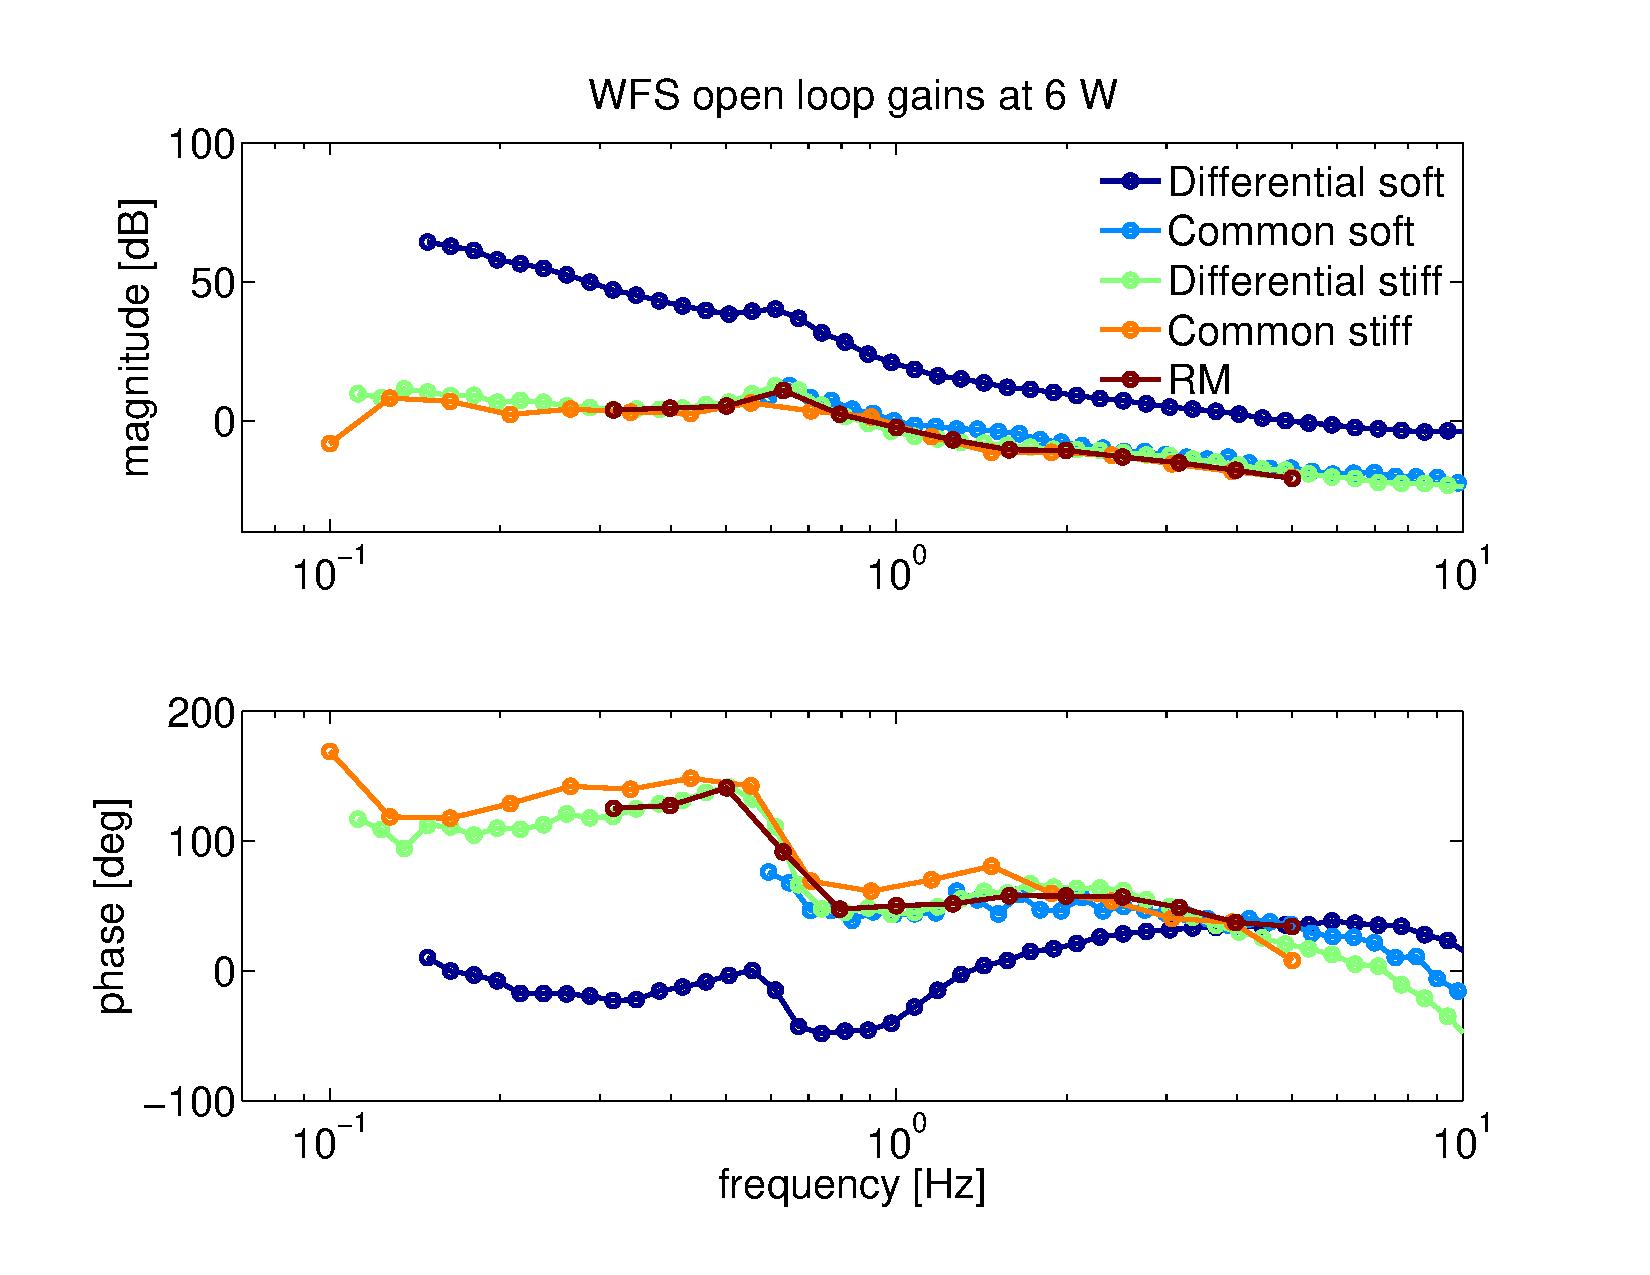
\includegraphics[width=0.8\columnwidth]{figures/olgs6W.pdf}
\subfigure{\includegraphics[width=1.0\columnwidth]{figures/allolgs_6W_mags.pdf}}
\subfigure{\includegraphics[width=1.0\columnwidth]{figures/allolgs_6W_phases.pdf}}
\caption{Open loop gains (pitch) of the 5 WFS loops as measured with 6 W
  input power.}
\label{fig:olgs6W}
\end{centering}
\end{figure}


% \begin{figure}
% \begin{centering}
% \subfigure{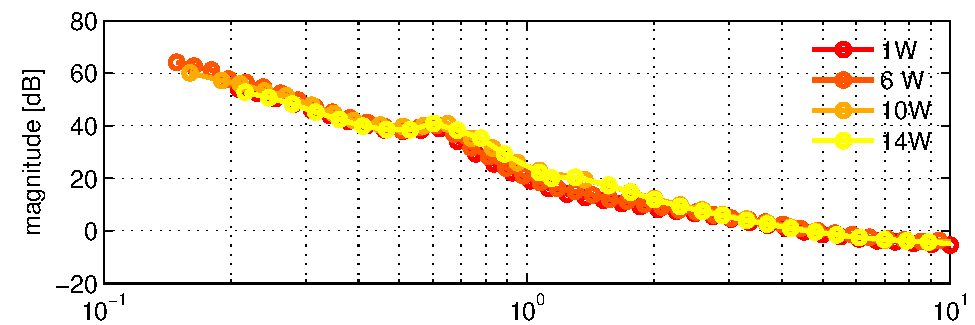
\includegraphics[width=1.0\columnwidth]{figures/wfs1_olgs_mags.pdf}}
% \subfigure{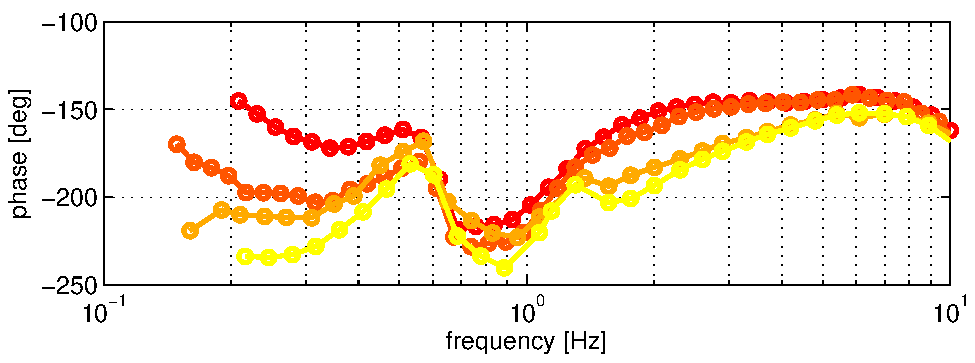
\includegraphics[width=1.0\columnwidth]{figures/wfs1_olgs_phases.pdf}}
% \caption{Open loop gains (pitch) of the differential soft (WFS1) loop as measured at four
%   different powers.}
% \label{fig:DSolgs}
% \end{centering}
% \end{figure}

% \begin{figure}
% \begin{centering}
% \subfigure{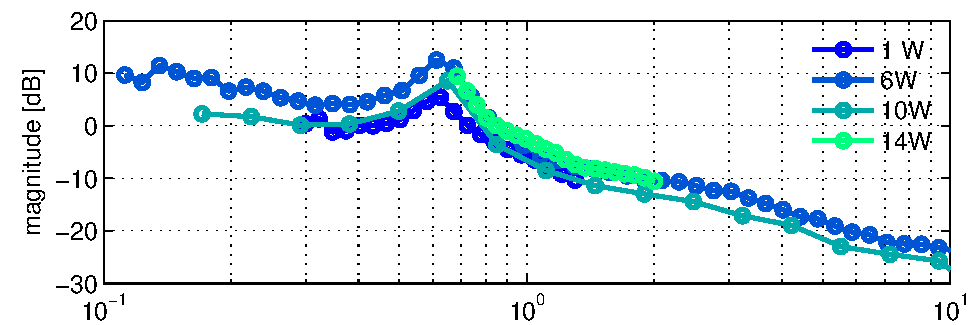
\includegraphics[width=1.0\columnwidth]{figures/wfs2b_olgs_mags.pdf}}
% \subfigure{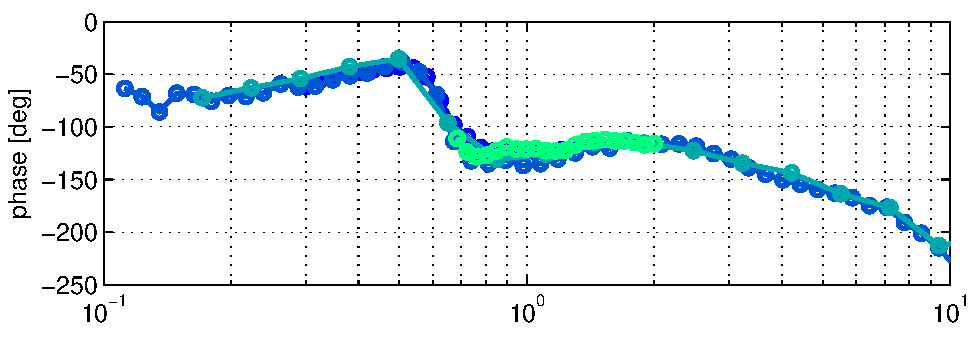
\includegraphics[width=1.0\columnwidth]{figures/wfs2b_olgs_phases.pdf}}
% \caption{Open loop gains (pitch) of the differential hard (WFS2B) loop as measured at four
%   different powers.}
% \label{fig:DHolgs}
% \end{centering}
% \end{figure}




\section{Residual Angular Motion}
The residual beam spot motion is shown in Fig.~\ref{fig:bsm}. We see
the rms beam spot motion on the ETMs is 1~mm and on the ITMs it is
0.8~mm. This meets the requirements of Sec.~\ref{sec:tolerance}.

\begin{figure}
\begin{centering}
\subfigure{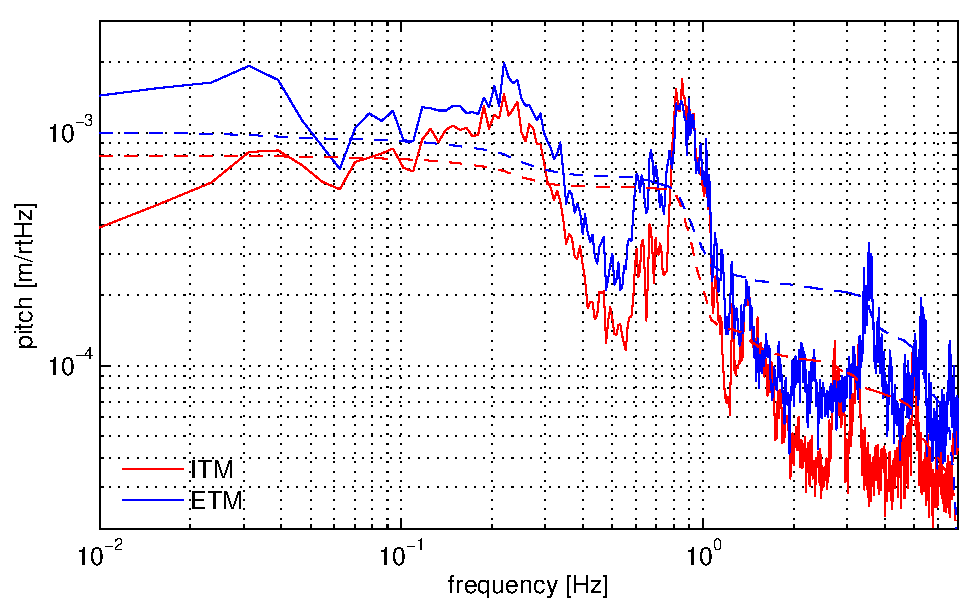
\includegraphics[width=1.0\textwidth]{figures/BSMpit.pdf}}
\subfigure{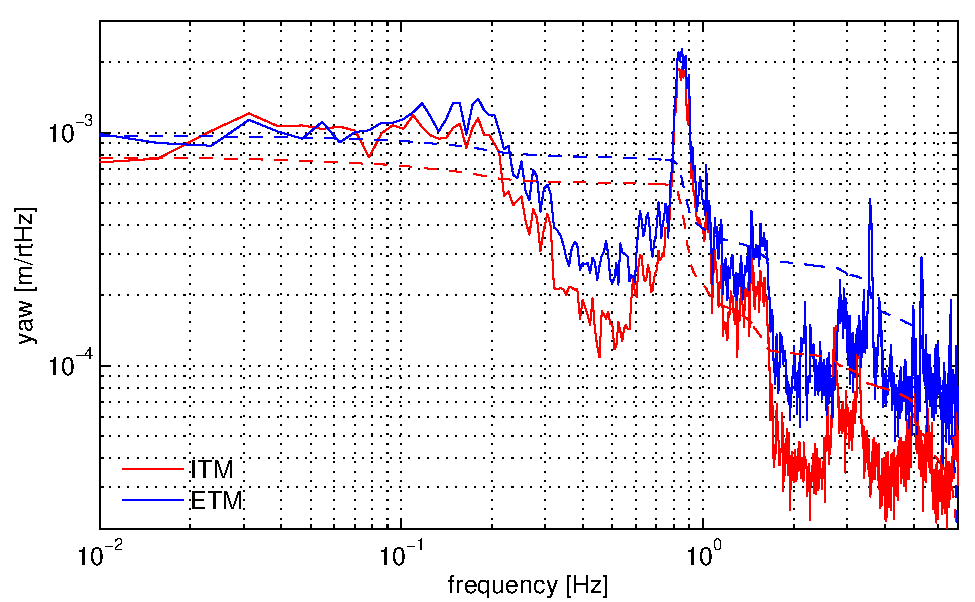
\includegraphics[width=1.0\textwidth]{figures/BSMyaw.pdf}}
\caption[Beam spot motion on the ITMs and ETMs during a 16~W
lock]{Beam spot motion on the ITMs and ETMs during a 16~W lock at
  night. Ground motion at the time of this measurement is shown in
  Fig.~\ref{fig:seismic_bsm}}%(May21, 2010, 06:02:30 UTC).}
\label{fig:bsm}
\end{centering}
\end{figure}


% \begin{figure}
% \begin{centering}
% \subfigure{\includegraphics{figures/DS_darkres.pdf}}\subfigure{\includegraphics{figures/CS_darkres.pdf}}
% \subfigure{\includegraphics{figures/DH_darkres.pdf}}\subfigure{\includegraphics{figures/CH_darkres.pdf}}
% \subfigure{\includegraphics{figures/RM_darkres.pdf}}
% \caption[Residual motion of the radiation pressure eigenbasis degrees
% of freedom]{Residual motion of the radiation pressure eigenbasis
%   degrees of freedom using calibrated WFS error signals during a 10~W
%   lock compared to dark noise and the background motion as calculated
%   using the open loop transfer function measurements. The sensor dark
%   noises (see Fig.~\ref{fig:WFSdarknoise}) are put in the RP
%   eigenbasis by propagation through the WFS power scaling and WFS
%   input matrix. Ground motion at the time of the residual motion
%   spectra is found in Fig.~\ref{fig:seismic_locked}.}
% \label{fig:WFSresidual}
% \end{centering}
% \end{figure}

We quantify the effect of the ASC on the radiation pressure eigenbasis
degrees of freedom by comparing spectra of the residual eigenbasis
motion during lock to the equivalent eigenbasis motion as witnessed by
the optical levers out of lock. The comparisons cannot be perfect
because the spectra are necessarily taken at different times and
therefore with different seismic noise conditions. However, the effect
of the ASC is stark at low frequencies where gain is high, as is seen
in Figure~\ref{fig:ASConoff}. At 0.01~Hz angular motion of all degrees
of freedom is suppressed by at least one order of magnitude. The
typical residual rms angular motion is $10^{-7}$
rad/$\sqrt{\mathrm{Hz}}$. The effect of the high gain for the
differential soft degree of freedom, in particular, is seen here,
where order of magnitude suppression is seen already at 1~Hz.

\begin{figure}
\begin{centering}
\subfigure{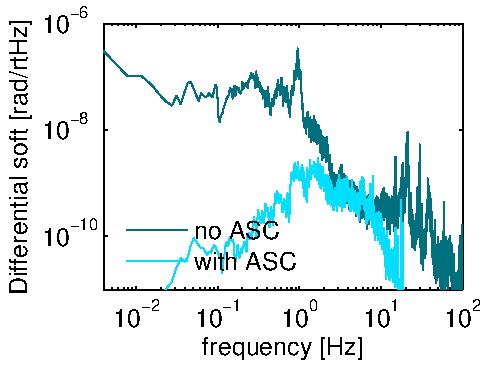
\includegraphics[width=0.5\textwidth]{figures/onoff_DS.pdf}}\subfigure{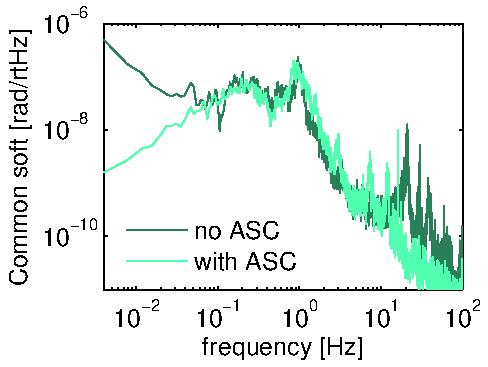
\includegraphics[width=0.5\textwidth]{figures/onoff_CS.pdf}}
\subfigure{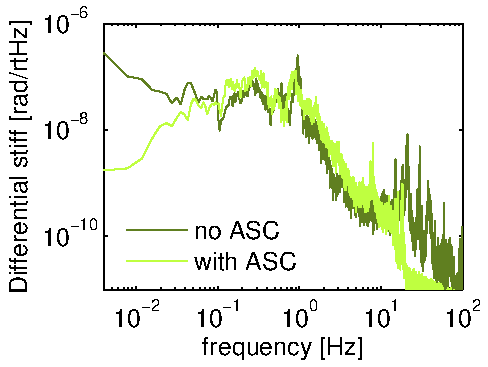
\includegraphics[width=0.5\textwidth]{figures/onoff_DH.pdf}}\subfigure{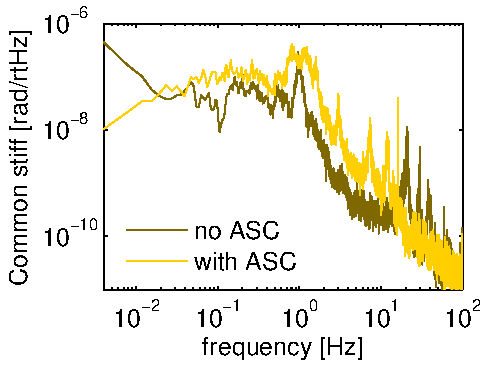
\includegraphics[width=0.5\textwidth]{figures/onoff_CH.pdf}}
\subfigure{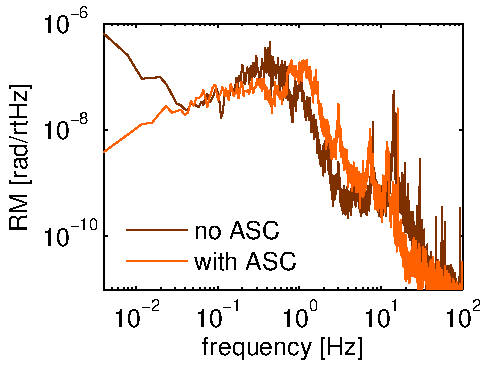
\includegraphics[width=0.5\textwidth]{figures/onoff_RM.pdf}}
\caption[Angular motion suppression due to the ASC]{Demonstration of
  angular motion suppression down to 4~mHz due to the ASC. 
%Same as Fig.~\ref{fig:WFSresidual}, but the background (here called
%``no  ASC'') 
The background motion (``no ASC'') is the RP eigenbasis reconstruction of optical lever signals
  when the interferometer is not locked. Data are taken 45 minutes
  apart, and the ground motions are shown in
  Figures~\ref{fig:seismic_nolock} and \ref{fig:seismic_locked}. The
  differences in ground motion explains the discrepancies between 1~Hz
  and 10~Hz.}
\label{fig:ASConoff}
\end{centering}
\end{figure}

The magnitudes of the beam spot motion and the residual mirror motion
are consistent and reasonable. For example, for $10^{-7}$ rad of soft
or hard mode motion in one arm, the maximum cavity tilt and
displacement are (from Table.~\ref{table:cav_geometric})
0.12~\micro rad and 1.02~mm, respectively.


Figure~\ref{fig:mirror_onoff} shows the same data as
Fig.~\ref{fig:ASConoff} except in the mirror basis instead of the
radiation pressure eigenmode basis. The ASC on/off comparison of
mirror motion is interesting because it shows that the mirrors
actually move more with respect to the ground when they are controlled
by the ASC than when they are not controlled by the ASC. This is to be
expected because the ground motion is different at each mirror and the
job of the ASC is to control the motions of the mirrors with respect
to each other, not with respect to the ground.

\begin{figure}
\begin{centering}
\subfigure{\includegraphics{figures/onoff_ITMX.pdf}}\subfigure{\includegraphics{figures/onoff_ITMY.pdf}}
\subfigure{\includegraphics{figures/onoff_ETMX.pdf}}\subfigure{\includegraphics{figures/onoff_ETMY.pdf}}
\subfigure{\includegraphics{figures/onoff_RMmir.pdf}}
\caption[Individual mirror motion with and without ASC]{Individual
  mirror motion with and without the ASC. The mirrors move more with
  respect to their local grounds when the interferometer is controlled
  than when they're on their own. Data are taken 45 minutes apart, and the ground
  motions are shown in Figures~\ref{fig:seismic_nolock} and
  \ref{fig:seismic_locked}.}
\label{fig:mirror_onoff}
\end{centering}
\end{figure}



% \begin{figure}
% \begin{centering}
% 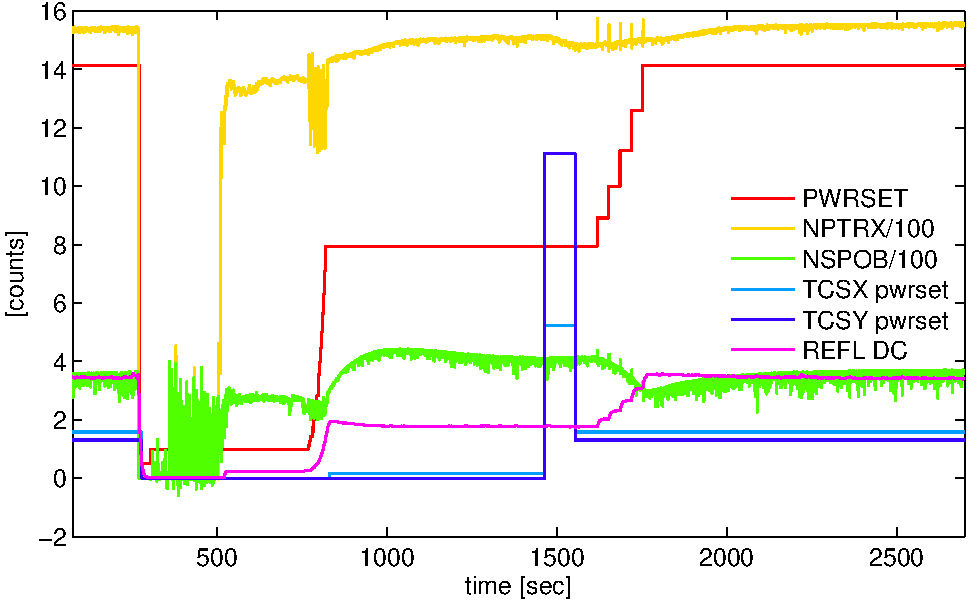
\includegraphics[width=1.0\columnwidth]{figures/timeseries_ifolocked.pdf}
% \caption[Striptool example]{Time series of interferometer signals
%   showing a typical lock loss and re-lock followed by an increase of
%   power to 14~W.} 
% % (From July 23, 2009 elog.) \textcolor{blue}{work this in somewhere.}}
% \label{fig:striptool}
% \end{centering}
% \end{figure}




\section{ASC to DARM Noisebudget}
One of the most important figures of merit of ASC performance is how
much noise the ASC contributes to DARM. We measure the coupling of the
ASC to DARM by injecting broadband noise between 40 and 110 Hz in each
of the suspension angular excitation
points\footnote{ie. \texttt{L1:SUS-ETMX\_ASCPIT\_EXCMON}} and
recording both the suspension angular control
signal\footnote{ie. \texttt{L1:SUS-ETMX\_ASCPIT\_OUT}} and
DARM. Signals from a time without excitation are subtracted from those
with the excitation, resulting in just the contribution to each
spectra due to noise. Dividing the noisy DARM spectrum by the noisy
suspension control spectrum provides the transfer function we use to
mulitiply by a suspension signal at any time. 

% \begin{figure}
% \begin{centering}
% \includegraphics[width=1.0\columnwidth]{figures/ASC2DARM_TFs.pdf}
% \caption[Measured ASC to DARM transfer functions]{ASC to DARM transfer
%   function for four of the five wavefront sensor loops. The RM to DARM
%   transfer function could not be measured because the contribution is
%   so small. The fitted curves can be multiplied by the WFS error
%   signals at any time to calculate the ASC noise contribution to
%   DARM. \textcolor{blue}{Need to turn cts into radians.}}
% \end{centering}
% \end{figure}

Figure~\ref{fig:optic2DARM} shows the result of applying the measured
ASC to DARM transfer function to each of the optic's angular control signals at
a time when the interferometer was locked with 14~W input power.

\begin{figure}
\begin{centering}
\subfigure[Pitch.]{\includegraphics{figures/opticspittoDARM.pdf}}
\subfigure[Yaw.]{\includegraphics{figures/opticsyawtoDARM.pdf}}
\caption[Optic to DARM noisebudget]{Optic to DARM noisebudget during a
  14~W lock.}% (July 17, 2009).
\label{fig:optic2DARM}
\end{centering}
\end{figure}

\begin{figure}
\begin{centering}
\subfigure[Pitch.]{\includegraphics{figures/WFSpittoDARM.pdf}}
\subfigure[Yaw.]{\includegraphics{figures/WFSyawtoDARM.pdf}}
\caption[Wavefront sensor to DARM noisebudget]{Wavefront sensor to
  DARM noisebudget during a 14~W lock.} % (July 17, 2009).}
\label{fig:wfs2DARM}
\end{centering}
\end{figure}

We also repeated the transfer function measurement with excitations
and readback not at the suspension angular control point, but at the
WFS error points. This allows us to view the breakdown of noise
contributions in the WFS (radiation pressure eigenmode) basis rather
than the optic basis. Figure~\ref{fig:wfs2DARM} shows the breakdown of
WFS noise contributions to DARM for the same time as
Fig.~\ref{fig:optic2DARM}.

Because two angular control signals, the WFS and the optical levers,
independently contribute signals to the suspension angular control, we
can separate their contributions in the noisebudget. Furthermore, we
compute the quadrature sum of the pitch and yaw contributions,
assuming these two degrees of freedom are de-coupled, thus creating an
upper limit for the ASC contribution to the DARM
noisebudget. Figure~\ref{fig:asc2darm} shows the final ASC noise in
DARM summary for a 16~W lock at night.

\begin{figure}
\begin{centering}
\includegraphics[width=1.0\columnwidth]{figures/ASC2DARM.pdf}
\caption[Total WFS and optical lever noise contribution to DARM during
a 16 W lock at night]{Total WFS and optical lever noise contribution
  to DARM during a 16 W lock at night. Pitch and yaw contributions are
  added in quadrature under the assumption they are
  de-coupled. Seismic spectra at the time of this measurment are found
  in Fig.~\ref{fig:seismic_NB}.}
\label{fig:asc2darm}
\end{centering}
\end{figure}

The important message is that the angular sensing and control is, in
fact, a limiting noise source for frequencies between 20~Hz and
55~Hz. The ASC becomes less and less of a primary noise source as
frequency increases, and by 100~Hz the ASC noise floor is a factor of
10 below DARM. The seismic noise contribution to DARM (not shown) does
in fact sit just below the ASC floor, so the sensitivity is not
dramatically hindered by the ASC. An example, however, that
demonstrates how we can reduce the ASC noise floor, if only by a small
amount, is presented in the next section.



\subsection{Tuning the Cut-off Filters} 

\begin{figure}
\begin{centering}
\includegraphics[width=1.0\textwidth]{figures/cutoffWFS1_DARMcompare.pdf}
\caption[Effect of the WFS1 lowpass filter cutoff frequency on strain
sensitivity.]{Effect of the WFS1 lowpass filter cutoff frequency on
  strain sensitivity.}
% \textcolor{blue}{gray legend line missing?}}
\label{fig:WFS1cutoff}
\end{centering}
\end{figure}

The cut-off frequency of the lowpass filters for the WFS control are
of particular importance in the DARM noisebudget. The lowpass filter
is necessary for suppressing the impression of sensing noise on
suspension control signals. Steepening the cut-off frequency results
in less sensing noise impression, but each pole used to achieve the
steeper drop-off introduces an extra $90^{\circ}$ of phase
loss. Likewise, lowering the cut-off frequency reduces noise
impression, but it pushes the phase loss to lower
frequencies. Decreasing the phase margin of the WFS loops leads to
gain peaking and a greater likelihood of loop instability. A fine
balance must therefore be found between loop stability and noise
impression. Figure~\ref{fig:WFS1cutoff} demonstrates the effect on
DARM of decreasing the WFS1 cutoff filter frequency from 35~Hz to
30~Hz.





% \section{Feed-Forward}
% Implementing a method of Wiener filtering, I show that the angular
% sensing and control error signals can be predicted by ground motion
% witnessed by local seismometers.

% Using S6 data, I evaluated the potential benefits of seismic
% feed-forward for the angular degrees of freedom. I designed FIR Wiener
% filters from simultaneous seismometer and ASC error signal time
% series. The Wiener filter minimizes the mean square error between the
% ASC error signal and the Wiener filtered seismometer data. The
% filtered seismometer data can be a good approximation to the ASC error
% signal and thus fed-forward. I found that with a sufficiently long
% Wiener filter and 30 minutes worth of data, we can accurately predict
% the ASC error signal from 0.1 to 20 Hz. If implemented, the rms
% angular mirror motion would be reduced by a factor of ten and yield a
% potential reduction in DARM at low frequencies. More importantly, less
% angular mirror motion would make for a more stable interferometer,
% necessary for high power operation, a key challenge for aLIGO.

% \textcolor{blue}{put in Wiener filter figures; explain Wiener
%   filtering or reference?}

% \section{Advanced LIGO}
% The Advanced LIGO interferometers will have more massive mirrors, a stable
% recycling cavity, and more circulating power. 





\section{Experimental measurement of the Sidles-Sigg effect}

\begin{figure}
\begin{centering}
\includegraphics[width=1.0\textwidth]{figures/ascservo_measurement.pdf}
\caption[Demonstration of radiation pressure eigenbasis torque to
  angle transfer function measurement]{Demonstration of radiation pressure eigenbasis torque to
  angle transfer function measurement. Through a proper choice of measurement
  locations within the ASC servo, the plant's transfer function can be
  singled out.}
\label{fig:RPTFmeasurement}
\end{centering}
\end{figure}

The digital control system in which the angular control feedback
system is implemented provides a convenient milieu in which to measure
the response of the optomechanical system.  By injecting a disturbance
somewhere in the loop and measuring the response at selected points in
the loop, we can produce a measurement of the optomechanical system
that is not sensitive to the details of the control system.   Here we
use this system to produce measurements of the optomechanical plant at
several different operating powers, demonstrating the modifications due
to radiation pressure, i.e. the Sidles-Sigg effect.

The various elements of the plant and the control system are depicted
in figure~\ref{fig:RPTFmeasurement}.  For this measurement, transfer
functions are taken from torque input to the resulting angular
displacement (as measured by the WFS), both in the radiation pressure
eigenbasis.  Simultaneously, an excitation is injected into the
control leg of the servo loop.  The resulting measurement reproduces
the transfer function of the optomechanical plant, independent of the
control system.

Results are shown in figures~\ref{fig:hardTF} (hard mode) and
~\ref{fig:softTF} (soft mode); least-squares fits of second-order
transfer functions are made to the data.  In the hard mode plot, we
can clearly see the increase of the resonant frequency with power,
from $\sim0.65$ Hz at 1~W input power to $\sim0.95$ Hz at 10~W input
power.  Simultaneously, in the soft mode plot, we see the resonance
decrease in frequency as the power is increased from 1~W to 6~W.  When
the input power is increased to 10W and beyond, the resonance
disappears; the plant has become statically unstable.

\begin{figure}
\begin{centering}
\subfigure{\includegraphics{figures/hardmag.pdf}}
\subfigure{\includegraphics{figures/hardphase.pdf}}
\caption{Hard opto-mechanical mode measurement and fit for several
 powers.}
\label{fig:hardTF}
\end{centering}
\end{figure}

\begin{figure}
\begin{centering}
\subfigure{\includegraphics{figures/softmag.pdf}}
\subfigure{\includegraphics{figures/softphase.pdf}}
\caption{Soft opto-mechanical mode measurement and fit for several
 powers.}
\label{fig:softTF}
\end{centering}
\end{figure}

These measurements show a clear confirmation of the Sidles-Sigg theory
and demonstrate a successful power-independent diagonalization of the
sensing and control of the optomechanical system.

% \section{Summary}
% \textcolor{blue}{from Guido: add another summary here that ASC in
%   neither base was limiting us but that the experience gained for
%   aLIGO is priceless. Some catch phrase that highlights a particular
%   lesson learned would be good}








% \section{Calibrations}
% Since the data is collected digitally, the units are in digital
% counts. This must be converted into physical units in order to
% facilitate comparison to models and to make meaningful statements. The
% typical method of calibrating a digital channel is to inject a signal
% of known amplitude into the system and take the ratio with the
% amplitude of the digital measurement of the signal. Two ways of
% determining the physical amplitude of the injected signal are
% \textcolor{blue}{(see if I can classify calibration methods)}
% \begin{itemize}
% \item 
% \item 
% \end{itemize}
% I describe in this section the calibrations I made of some of the
% angular sensing channels, all the while demonstrating particular
% examples of these methods.


% \subsection{Beam Spot Motion}
% A quantity of interest is how much the beam moves on the ITMs and
% ETMs. It is this beam spot motion which, together with the mirror
% angular motion, creates a length signal that contributes noise to
% DARM. An elegant way of following the motion of the beam on the test
% masses is to track pickoffs of the light transmitted or reflected from
% the mirrors. We have such signals naturally available for the ETMs and
% ITMs from the QPDs which are otherwise used for ASC sensing. For
% example, QPDX and QPDY see the light transmitted through each of the
% ETMs and WFS2 sees the pickoff of light from the wedge of ITMX.

% To calibrate the counts of the QPD and WFS2 pitch and yaw error
% signals,\footnote{\texttt{L1:ASC-QPDY\_\{PIT,YAW\}\_IN1} and
% \texttt{L1:ASC-WFS2\_DC\{Pitch, Yaw\}Mon}} I moved the beam a
% known distance on the test mass, $\Delta x$, and recorded the
% corresponding $\Delta y$ of the QPD and WFS2 readback. The ratio
% $\Delta x /\Delta y$ is the calibration from counts to meters. The
% details of the procedure are described below.


% \subsubsection{Moving the beam} 
% Moving the beam on the mirrors in a controlled fashion is
% straightforward because of the ASC system. All that we need to do is
% introduce an offset to the setpoint of the of the beam centering
% aspect of the ASC servo. For the ETMs we put a DC offset in the
% \texttt{L1:ASC-QPD\{X,Y\}\_\{PIT, YAW\}\_\{OFFSET\}} channel and for
% the ITMs we changed the $X$ and $Y$ targets of the beam splitter beam
% centering servo.

% \subsubsection{Measuring how much the beam has moved} 
% The more difficult task is measuring just how much the beam has
% moved. For this, we make use of the lever arm mechanism of angle to
% length coupling. \textcolor{blue}{(This should be explained in the
%   previous chapter, so maybe just reference it.)} The idea is that
% when the axis of rotation of a mirror coincides with the center of the
% beam, any tilt of the mirror about this axis does not affect the path
% length of the reflected beam. However, if there is a mismatch between
% rotation axis and beam location, then the light will pick up a
% longitudinal phase shift when the mirror is tilted. During a full
% interferometer lock, this is recorded by DARM.

% The concept of the measurement is to move the axis of rotation of the
% mirror so that it passes through the center of the beam. We use the
% OSEMs to change the location of the axis of rotation, and we use DARM
% to determine when the axis is aligned with the beam center. For
% example, if we drive the top two OSEMs more than the bottom two OSEMs,
% we've created an axis of rotation that sits below the center of
% mass. The result of such tuning is an effective rebalance of the
% center of mass of the mirror so that it is aligned with the center of
% the beam. The procedure is:
% \begin{enumerate}
% \item Shake the mirror at some frequency $f$ (we use
% 39.5 Hz) during a full lock \vspace{-10pt}
% \item Demodulate DARM at $f$ for several different sets of OSEM gains \vspace{-10pt}
% \item Fit a quadratic to the demodulated data to pinpoint the OSEM gains that
%   minimize the coupling to DARM
% \end{enumerate}

% \begin{figure}
% \begin{centering}
% \includegraphics[width=0.5\columnwidth]{figures/geometry_mirror_osems.pdf}
% \caption[Diagram of mirror and OSEM geometry]{Geometry of OSEMs and
%   mirror as used for calculating the location of the axis of rotation
%   when the torques are unequal. \textcolor{blue}{Need latex in
%     inkscape!}}
% \label{fig:mirror_osem_geometry}
% \end{centering}
% \end{figure}

% Relating the OSEM gains to absolute beam position on the mirror
% requires only the geometry of the mirror and OSEM setup as sketched in
% Fig. \ref{fig:mirror_osem_geometry}. We estimate the OSEM locations as
% being on the edge of the mirror such that the length $d$ of one side
% of the square that they form is given by $d =\sqrt{2} R$, where $R =
% 12.5$ cm is the radius of the mirror. Then, collapsing the four OSEMs
% into a representative two at the centers of two opposite sides of the
% square and assigning them gains of $1 + \alpha$ and $-(1-\alpha)$ for
% a force $F$, we can evaluate where the pivot point $x$ is located by
% setting the sum of the torques equal to zero:
% \begin{equation}
% F [1+\alpha] x = F [1-\alpha][d-x].
% \end{equation}
% Therefore, the beam location relative to center, $\Delta x$, is
% \begin{equation}
% \Delta x := \frac{d}{2} - x = \alpha \frac{d}{2},
% \end{equation}
% and for a change in a pitch or yaw coil gain, the change in beam
% position, $\Delta x$, is:
% \begin{equation}
% |\Delta{x}| = \frac{|\Delta{\mbox{gain}}| R}{\sqrt{2}} .
% \end{equation}

% The final calibrations of these channels are shown in Table
% \ref{table:bsmcal}. \footnote{A minor technicality is that since there
%   are no filters between the QPD error signals and the offset channel,
%   their units are exactly the same. Thus, calculating meters of beam
%   spot motion as a function of offset serves to calibrate the error
%   point. For convenience, this is what I did.}

% \begin{table}
% \centering
% \caption[Beam spot motion calibrations]{Calibrations to be used with
%  the QPDX, QPDY, and WFS2 DC pitch and yaw error signals for a
%  measure of beam spot motion.} 
% \begin{tabular}{l l l l}
% \hline
%          & ETMX & ETMY & ITMs \\
% \hline
% pitch & 1.03e-5 m/ct & 1.21e-5 m/ct & 5.52e-2 m/ct \\
% yaw & 0.88e-5 m/ct & 0.80e-5 m/ct & 4.79e-2 m/ct \\
% \hline
% \end{tabular}
% \label{table:bsmcal}
% \end{table}



% \subsection{Angular Mirror Motion}
% The optical levers provide a straightfoward measure of individual
% mirror motion. The channels I calibrated were of the form
% \texttt{L1:SUS-ETMX\_OPLEV\_\{P,Y\}ERROR}, the optical lever error
% signals for each of the large optics. I made use of the dependence of
% power in a misaligned cavity to calibrate the ETM and ITM optical
% levers, and used a less precise, rudimentary method to calibrate the
% RM, BS, and MMT3 optical levers.


% \subsubsection{ETM and ITM optical levers} 
% I calibrated the arm cavity optical levers by tracking the power loss
% in the locked arm as one of its mirrors is tilted. The closed form
% expression for cavity power as a function of mirror tilt is derived in
% Appendix \ref{sec:cavitypower}. All that is needed is a quadratic fit
% to the data collected. From the fit parameters, I can determine the
% factor, $\Delta \theta / \Delta y$, which converts the digital counts
% of the optical lever channel, $y$, to units of radians.

% To make the measurement, I locked a single arm and maximized the power
% build up. Then I slowly stepped the pitch or yaw pointing of one of
% the mirrors away to one side of resonance, and then back and to the
% other side, repeating this several times. All the while, I recorded
% the optical lever error signal of the mirror whose angle I was
% changing, and the power in the arm as determined from the amount of
% light transmitted through the
% ETMs.\footnote{\texttt{L1:LSC-NPTR\{X,Y\}\_OUT16}}

% From Eq.~\ref{eq:pwr_disptilt}, we see that the power in the arm, $P$,
% is a function of the form 
% \begin{equation}
% P = P_{max} \exp{[-b (y-y_0)^2]},
% \label{eq:OLcalfit}
% \end{equation}
% where $y_0$ is the DC offset of the optical lever channel and $b$ is
% related to physical cavity axis displacement $a$ and tilt $\alpha$ by
% $by^2~=~(a/w_0)^2+(\alpha/\theta_0)^2$. In order to relate the optical
% lever signal, $y$, to physical cavity parameters, we divide by
% $\Delta{\theta}^2$ and rearrange to get:
% \begin{equation}
% \frac{\Delta \theta}{\Delta y} = \sqrt{b} \left[
%   \left[\frac{\Delta a/\Delta\theta}{w_0}\right]^2 +
%   \left[\frac{\Delta\alpha/\Delta\theta}{\theta_0}\right]^2
% \right]^{-\frac{1}{2}} .
% \end{equation}
% The terms in the numerators on the right hand side are fixed constants
% based on the cavity geometry and can be calculated using
% Eq. \ref{eq:cavitydisptilt_mirrorangle}. The measurement data and fits
% are shown for both pitch and yaw in Fig. \ref{fig:OLcal}. The ETM
% optical levers make use of a broader range of optical lever signal
% than do the ITMs. (Also note that the maximum power in the y-arm is about
% 10\% less than that in the x-arm. This is true at both Hanford and
% Livingston, and is due to the priority given to the x-arm in the
% alignment scheme, as explained in Appendix
% \ref{sec:initial_alignment}.)

% \begin{figure}
% \begin{centering}
% \subfigure{\includegraphics[width=0.5\columnwidth]{figures/olcal_pitch.pdf}}\subfigure{\includegraphics[width=0.5\columnwidth]{figures/olcal_yaw.pdf}}
% %\includegraphics[width=1.0\columnwidth]{figures/oplevcal_pitch.pdf}
% \caption[Optical lever calibration data.]{Optical lever calibration data and
%   fits to Eq. \ref{eq:OLcalfit}.}
% \label{fig:OLcal}
% \end{centering}
% \end{figure}


% \subsubsection{RM, BS, and MMT3 optical levers}
% To calibrate the RM, BS and MMT3 optical levers, I used my own eyes
% and the camera images and known dimensions of the ETM beam cages. With
% the interferometer unlocked, I moved the optics in pitch and yaw,
% tracking the beam's movement on the ETM cages. In order to calibrate
% the RM, I used the reflection off ITMY to the RM and onto the ETMY
% cage. The BS and MMT3 required only straight shots to the ETMs. For
% yaw, I moved the mirrors until the beam was centered on each vertical
% suspension post, and for pitch I moved the beam from the center of the
% mirror to the top of the cage. The beam moves by $x = 2\theta$ on
% across the cage when the mirror moves by $\theta$, so with small angle
% approximations, the mirror angle is simply $x/2L$ where $L$ is the
% distance from mirror to ETM cage.

% The final $\Delta\theta / \Delta x$ calibrations of all optical levers
% are in Table \ref{table:oplevcal}. 

% \begin{table}
% \centering
% \caption[Optical lever calibrations]{Calibrations to be used
%   with the optical lever error signals 
%   for a measure of angular mirror motion. Units are \microrad/ct.}
% \begin{tabular}{l l l l l l l l}
% \hline
%         & ETMX & ETMY & ITMX & ITMY & RM & BS & MMT3 \\
% \hline
% pitch & 49.4 & 43.0 & 14.9 & 15.6 & 61.9 & 47.3 & 57.4 \\
% yaw & 50.7 & 43.3 & 20.1 & 20.2 & 42.5 & 63.5 & 55.5 \\
% \hline
% \end{tabular}
% \label{table:oplevcal}
% \end{table}





% \subsection{WFS Error Signals}
% The WFS error signals (i.e. \texttt{L1:ASC-WFS1\_Q1}) are physically
% Watts of power at the detectors, which the WFS electronics convert
% into a voltage. To turn WFS counts into voltage of signal at the
% output of the detector, we must backtrack through the electronics and
% calibrate the WFS demodulation chain.

% % The WFS error signals (i.e. \texttt{L1:ASC-WFS1\_Q1}) are physically
% % Watts of power at the detectors. Converting the error signal in
% % digital counts to Watts requires working backwards through the
% % electronics, and can be divided into two parts. First, we must
% % calibrate the WFS demodulation chain to backtrack WFS counts into
% % voltage of signal at the input to the mixer. Second, we must convert
% % voltage at the mixer into Watts at the sensor based on properties of
% % the photodetector RF electronics. \textcolor{blue}{For now, it
% %   suffices to calibrate the signal in Volts.}

% %\subsubsection{Counts to Volts} 
% The analog to digital RF chain for the WFS includes a demodulation
% board, a whitening board, an anti-alias board, and the ADC. This chain
% can be calibrated by injecting a sine wave of the same frequency as a
% typical WFS signal, yet of known voltage into the WFS demodulation
% board. Comparing the peak to peak voltage of this input sine wave to
% the peak to peak amplitude of the resulting digital counts signal
% provides the Volts per count conversion. The calibrations are
% presented in Table \ref{table:demodcal}.

% \begin{table}
% \centering
% \caption[Demodulation chain calibration for each quadrant of each
%  WFS]{Demodulation chain calibration for each quadrant of each
%  WFS. Units are \micro V/count.}
% \begin{tabular}{l l l l l l}
% \hline
%  & q1 & q2 & q3 & q4 & average \\
% \hline
%  WFS1  & 0.35 &   0.32 &   0.34 &   0.35 & 0.34 \\
%  WFS2  & 8.8 &   8.6 &   8.7  &  8.5 & 8.7       \\
%  WFS3  & 6.4 &   5.8 &   5.8 &   5.7 & 5.9     \\
%  WFS4  & 6.3 &   5.4 &   5.3  &  7.4 & 6.1    \\
% \hline
% \end{tabular}
% \label{table:demodcal}
% \end{table}

% It should be noted that the demodulation chain calibration numbers for
% all quadrants of a particular WFS differ no more than 20\% from the
% average. The demodulation chain does not significantly distort the
% error signals.


% % \subsubsection{Volts to Watts}
% % The voltage created per Watt of signal on the WFS is determined by the
% % responsivity (Amps/Watt) and transimpedance (Volts/Amp) of the
% % diode. A model of the 25~MHz WFS transimpedance is shown in
% % Fig. \ref{fig:wfs25MHzTF}, indicating a magnitude of 90~dB at
% % 25~MHz. The responsivity is found in Section \ref{sec:pds}. It is
% % 0.86~A/W. 

% % The final WFS calibration numbers are found in Table \ref{tab:WFScal}.

% % \begin{figure}
% % \begin{centering}
% % \includegraphics[width=1.0\textwidth]{figures/wfs25MHzTF.pdf}
% % \caption{Transimpedance of the 25 MHz resonant RF WFS front end
% %   electronics. The model was made using software called LISO.}
% % \label{fig:wfs25MHzTF}
% % \end{centering}
% % \end{figure}

% % \begin{table}
% % \centering
% % \caption[]{WFS error signal calibrations from digital counts to Watts.}
% % \begin{tabular}{l l l l}
% % \hline
% % WFS1 & WFS2 & WFS3 & WFS4 \\
% % \hline
% % $3.9\times10^{-16}$ & $1.0\times10^{-14}$ & & \\
% % \hline
% % \end{tabular}
% % \label{table:WFScal}
% % \end{table}



